\documentclass{article}
\usepackage[utf8]{inputenc}
\usepackage{booktabs}
\usepackage{multirow}

\title{EnergyFlowNetwork}
\author{}
\date{April 2020}

\usepackage{natbib}
\usepackage{graphicx}

\begin{document}

\maketitle

\section{Introduction}
Energy Flow Network(EFN) and Particle Flow Network(PFN) are algorithms that take jet constituents information as input. EFN takes the rapidity ${y}$ and azimuthal angle ${\phi}$ of jet constituents as input, while PFN takes the rapidity $y$, azimuthal angle $\phi$ and transverse momentum $p_{T}$ as input. 
By just feeding those basic information to the algorithm without doing any high level reconstruction, we can try to find out whether the learning algorithm can extract some useful information from the data.
The EFN and PFN are composed of two networks as shown in Figure \ref{fig:EFNArch}. 
We used 200 nodes for each hidden layer in network (a), 256 for latent space dimension and 300 nodes for each hidden layer in network (b). 

\begin{figure}[h!]
\centering
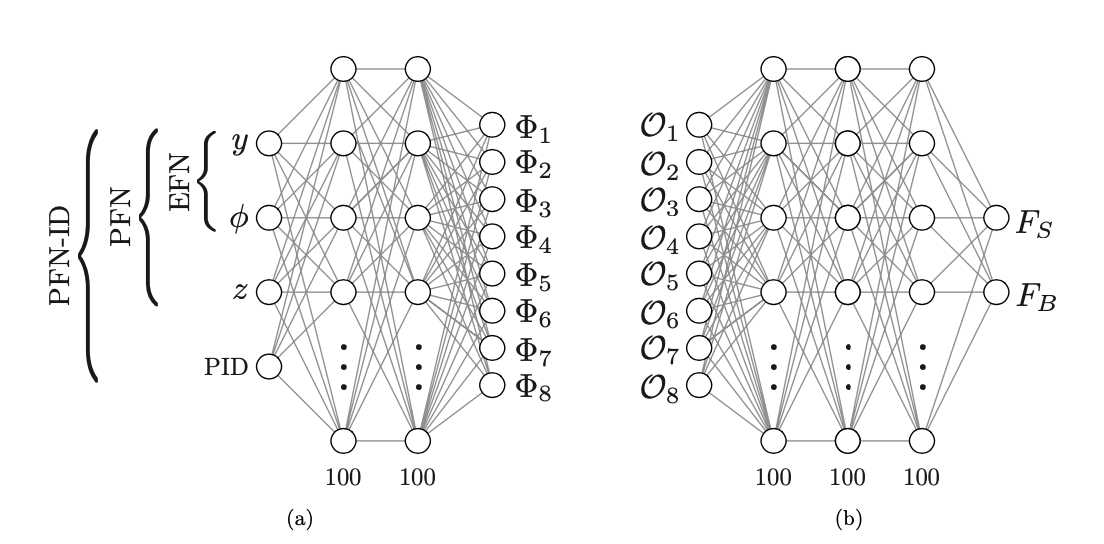
\includegraphics[scale=0.5]{EFNArch.png}
\caption{Network (a) takes jet constituents information as input and outputs latent space $\Phi$ for each jet constituents. Network (b) takes $\mathcal{O}$, which is the linear combination of $\Phi$, as input and outputs final result}
\label{fig:EFNArch}
\end{figure}

\section{Approach}
To test how the EFN and PFN works on diHiggs signal extraction. We generated 1M diHiggs events as signal and 4M QCD events as background. Also, we devided those events into four categories:
\begin{itemize}
    \item all events
    \item events with $ \geq $ 4 jets
    \item events with $ \geq $ 4 jets and 2 BTags
    \item events with $ \geq $ 4 jets and 4 BTags
\end{itemize}
We ran EFN and PFN using the events that belongs to those categories separately to see the performance of the learning algorithm. The number of backgrounds events that feed into the algorithm is adjusted to make the training balanced after the Jet and BTag cuts.
We used 60/20/20 data split as train/validation/test set.
To avoid overfitting, we tuned L2 regularization factor or dropout and applied early stopping.
To evaluate the performance, we calculated the signal significance for test set by $\frac{S}{\sqrt{B}}$ normalized to $3000fb^{-1}$ luminosity.

\section{Approach}
The results of EFN is shown in Table \ref{EFNtab} and the results of PFN is shown in Table \ref{PFNtab}
\begin{table}[h!]
\centering
  %\begin{center}
    \begin{tabular}{|l|c|c|c|} % <-- Alignments: 1st column left, 2nd middle and 3rd right, with vertical lines in between
      \hline\hline
      \multirow{2}{*}{\textbf{Category}} & \multicolumn{3}{c|}{0PU}\\
      \cline{2-4}
      & Best $S/\sqrt{B}$ & \textbf{N$_{\mathrm{Signal}}$} & \textbf{N$_{\mathrm{Background}}$} \\
      \hline
      All Events & $1.407 \pm 0.006$ & $1.89\cdot 10^4$ & $1.80\cdot 10^8$ \\
      4Jets & $1.363 \pm 0.006$ & $1.63\cdot 10^4$ & $1.43\cdot 10^8$ \\
      4Jets 2BTags & $1.343 \pm 0.006$ & $1.33\cdot 10^4$ & $9.95\cdot 10^7$ \\
      4Jets 4BTags & $0.867 \pm 0.008$ & $3468.65$ & $1.60\cdot 10^7$ \\
      \hline\hline
    \end{tabular}
    \caption{EFN results. Normalized to full HL-LHC dataset of 3000 fb$^{-1}$}
  %\end{center}
\label{EFNtab}
\end{table}

\begin{table}[h!]
\centering

  %\begin{center}
    \begin{tabular}{|l|c|c|c|} % <-- Alignments: 1st column left, 2nd middle and 3rd right, with vertical lines in between
      \hline\hline
      \multirow{2}{*}{\textbf{Category}} & \multicolumn{3}{c|}{0PU}\\
      \cline{2-4}
      & Best $S/\sqrt{B}$ & \textbf{N$_{\mathrm{Signal}}$} & \textbf{N$_{\mathrm{Background}}$} \\
      \hline
      All Events & $1.618 \pm 0.008$ & $1.79\cdot 10^4$ & $1.21\cdot 10^8$ \\
      4Jets & $1.580 \pm 0.008$ & $1.32\cdot 10^4$ & $7.00\cdot 10^7$ \\
      4Jets 2BTags & $1.574 \pm 0.009$ & $1.32\cdot 10^4$ & $4.85\cdot 10^7$ \\
      4Jets 4BTags & $0.903 \pm 0.009$ & $3297.34$ & $1.33\cdot 10^7$ \\
      \hline\hline
    \end{tabular}
    \caption{PFN results. Normalized to full HL-LHC dataset of 3000 fb$^{-1}$}
  %\end{center}
\label{PFNtab}
\end{table}



\bibliographystyle{plain}
\bibliography{references}
\end{document}
